\documentclass[11pt,twoside]{book}
\usepackage[mono=false]{libertine} % new linux font, ignore mono
\usepackage{luatex85}

\usepackage{amsmath,amsthm,amssymb,mathrsfs,amsfonts,dsfont}
\usepackage{epsfig,graphicx}
\usepackage{tabularx}
\usepackage{blkarray}
\usepackage{slashed}
\usepackage{color}
\usepackage{listings}
\lstset{
    language=bash,
    basicstyle=\ttfamily,
    breaklines=true,
    showstringspaces=false,
    commentstyle=\color{green!40!black},
    keywordstyle=\color{blue},
    stringstyle=\color{orange}
}
\usepackage{caption}
\usepackage{lipsum} % provides dummy text for testing
\usepackage[toc,title,titletoc,header]{appendix}
\usepackage{minitoc}
\usepackage{multicol} % two-col ToC
\usepackage{bm}
\usepackage{imakeidx} % before hyperref
\usepackage{hyperref}
\hypersetup{
    colorlinks=true,
    citecolor=magenta,
    linkcolor=black,
    filecolor=green,      
    urlcolor=cyan,
}
\usepackage[capitalise]{cleveref}
\usepackage{subcaption}
\usepackage{enumitem}
\usepackage{mathtools}
\usepackage{physics}
\usepackage[linesnumbered,ruled,vlined,algosection]{algorithm2e}
\SetCommentSty{textsf}
\usepackage{epigraph}
\epigraphwidth=1.0\linewidth
\epigraphrule=0pt

% adjust margin
\usepackage[margin=2.3cm]{geometry}
\headheight13.6pt

\usepackage{fancyhdr}
\pagestyle{fancy} % enable fancy page style
\renewcommand{\headrulewidth}{0.0pt} % comment if you want the rule
\fancyhf{} % clear header and footer
\fancyhead[lo,le]{\leftmark}
\fancyhead[re,ro]{\rightmark}
\fancyfoot[CE,CO]{\hyperref[toc-contents]{\thepage}}

\makeatletter
\def\chaptermark#1{\markboth{\protect\hyper@linkstart{link}{\@currentHref}{Chapter \thechapter ~ #1}\protect\hyper@linkend}{}}
\def\sectionmark#1{\markright{\protect\hyper@linkstart{link}{\@currentHref}{\thesection ~ #1}\protect\hyper@linkend}}
\makeatother

\usepackage[doi=false,url=false,isbn=false,style=alphabetic,backend=biber,backref=true]{biblatex}
\addbibresource{bib.bib}

\newbibmacro{string+doiurlisbn}[1]{%
  \iffieldundef{doi}{%
    \iffieldundef{url}{%
      \iffieldundef{isbn}{%
        \iffieldundef{issn}{%
          #1%
        }{%
          \href{http://books.google.com/books?vid=ISSN\thefield{issn}}{#1}%
        }%
      }{%
        \href{http://books.google.com/books?vid=ISBN\thefield{isbn}}{#1}%
      }%
    }{%
      \href{\thefield{url}}{#1}%
    }%
  }{%
    \href{http://dx.doi.org/\thefield{doi}}{#1}%
  }%
}

\DeclareFieldFormat[article,incollection,inproceedings,book,misc]{title}{\usebibmacro{string+doiurlisbn}{\mkbibemph{#1}}}
\DeclareFieldFormat{journaltitle}{#1\isdot}
\DeclareFieldFormat{booktitle}{#1\isdot}
\renewbibmacro{in:}{}
\DeclareSourcemap{
    \maps[datatype=bibtex]{
      \map{
        \step[fieldsource=video]
        \step[fieldset=usera,origfieldval]
    }
  }
}
\DeclareFieldFormat{usera}{\href{#1}{\textsc{Online video}}}
\AtEveryBibitem{
    \csappto{blx@bbx@\thefield{entrytype}}{% put at end of entry
        \iffieldundef{usera}{}{\space \printfield{usera}}
    }
}



% !TEX root = ./notes_template.tex

%%%%%%%%%%%%%%%%%%%%%%%%%%%%%%%%%%%%
%%%%%%%%%%%%%%%%%%%%%%%%%%%%%%%%%%%%
% math
\let\iff\relax
\newcommand{\iff}{\text{ iff }}
\newcommand{\OPT}{\textup{OPT}}

% physics
\newcommand{\acreation}{a^\dagger}



\usepackage[utf8]{inputenc}
\usepackage[spanish]{babel}
\addto\captionsspanish{\renewcommand{\figurename}{Figura}}

\begin{document}
% Portada
\begin{center}
  \LARGE UNIVERSIDAD DE LAS FUERZAS ARMADAS ESPE\\[0.5cm]
  \Large DEPARTAMENTO CIENCIAS DE LA COMPUTACIÓN \\[0.5cm]
  \large SISTEMAS OPERATIVOS\\[0.5cm]
  \begin{figure}[htb] \centering 
\includegraphics[scale=.6]{Logo_ESPE} \end{figure}
  \vspace{0.5cm}
  \large{\bf Consultas }\\ \vspace{.25cm}
\end{center}

\begin{flushleft}
  \Large{\bf NRC: } 14912 \textbf{}\\
  \vspace{0.5cm}
  \Large{\bf Carrera:} Ingeniería de Software\\
  \vspace{0.5cm}
  \Large{\bf Nombre: } Gustavo Aguas y Sebastian Paucar\\
  \vspace{0.5cm}
  \Large{\bf Docente: } Ing. Fuertes Diaz Walter Marcelo Dr.\\
  \vspace{0.5cm}
  %\Large{\bf Grupo: }
  \vspace{0.5cm}
\end{flushleft}

\begin{center} \Large \textsc{Sangolqui - Ecuador} \\
  \vspace{0.5cm}
  \Large \textsc{2024 } \end{center}
\let\cleardoublepage\clearpage

\chapter{Laboratorios}
\section{Laboratorio 1}
\subsection{Tema: Instalación, configuración y creación de una máquina virtual}

\textbf{Objetivos:}
\begin{itemize}
  \item Aprender a crear máquinas virtuales
  \item Crear nuestra primera máquina virtual
\end{itemize}

\textbf{Recursos:}
\begin{itemize}
  \item PC
  \item Windows 10
  \item VirtualBox
  \item Ubuntu - .ISO
\end{itemize}

\subsection*{Desarrollo}
Para realizar la practica de laboratorio tenemos que seguir los siguientes pasos:
\begin{enumerate}
  \item[\textbf{1.}] \textbf{Descargar la imagen de Ubuntu Desktop:} Acceder al sitio web oficial de Ubuntu y descargar la imagen de Ubuntu Desktop versión 24.04 LTS
  \item[\textbf{2.}] \textbf{Instalar Ubuntu Desktop: } Proceder con la instalación del sistema operativo utilizando la imagen descargada. Seguir cuidadosamente los pasos de instalación proporcionados por el asistente de instalación.
  \begin{enumerate}
    \item[\textbf{2.1}] Seleccionamos Normal Installation 
    \item[\textbf{2.2}] Seleccionamos el idioma que vamos a manejar y damos click en Install Ubuntu.
    \item[\textbf{2.3}] Por defecto nuestra localización Geográfica sera Guayaquil.
        \item[\textbf{2.4}] Ingresamos los datos que nos piden para continuar con la instalación.\\
\end{enumerate}
\item[\textbf{3.}] \textbf{Configurar Ubuntu Desktop}
\begin{enumerate}
    \item[\textbf{3.1}] Abrimos Virtual Box
    
    \begin{minipage}{\linewidth}
        \centering
        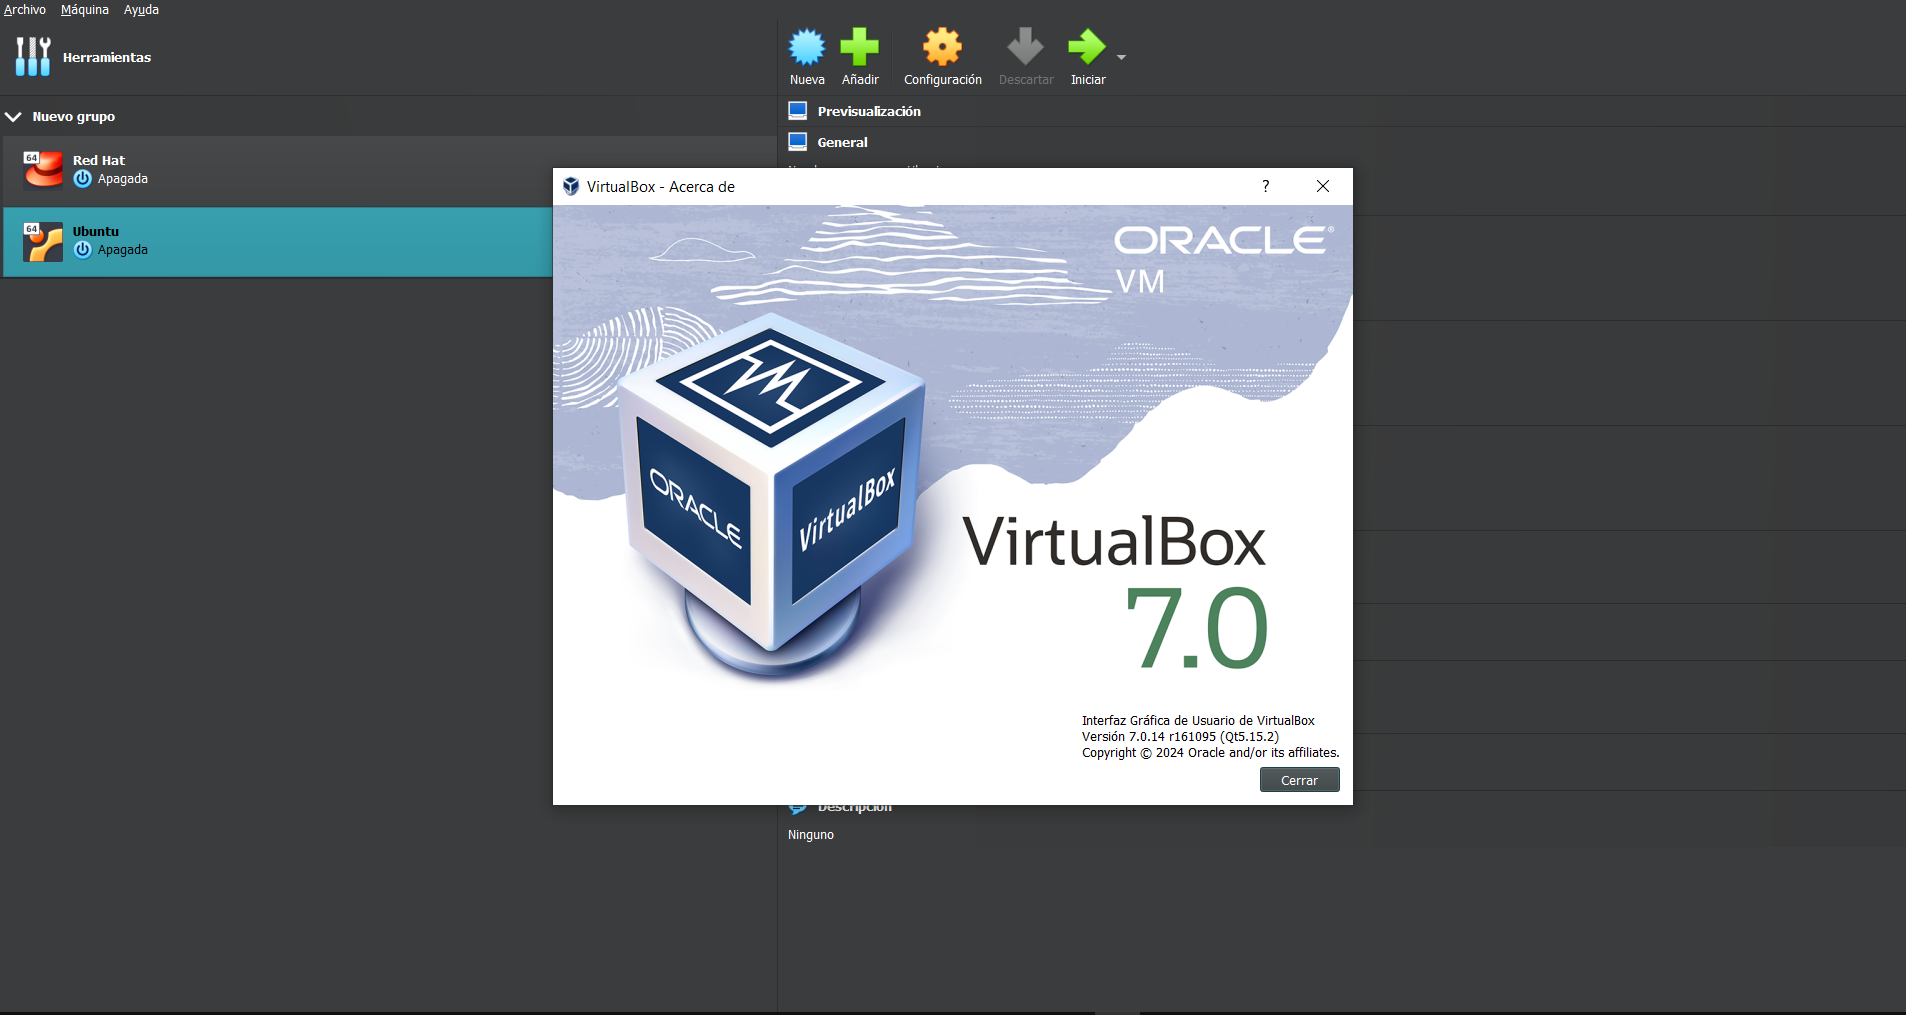
\includegraphics[width=0.5\linewidth]{VB.png}
        \captionof{figure}{Virtual Box}
        \label{fig:etiqueta}
    \end{minipage}\\
    
    \item[\textbf{3.2}] En la parte superior seleccionamos la opción Maquina y después la opción nueva, colocamos el nombre que deseamos para nuestra máquina virtual.
    
    \begin{minipage}{\linewidth}
        \centering
        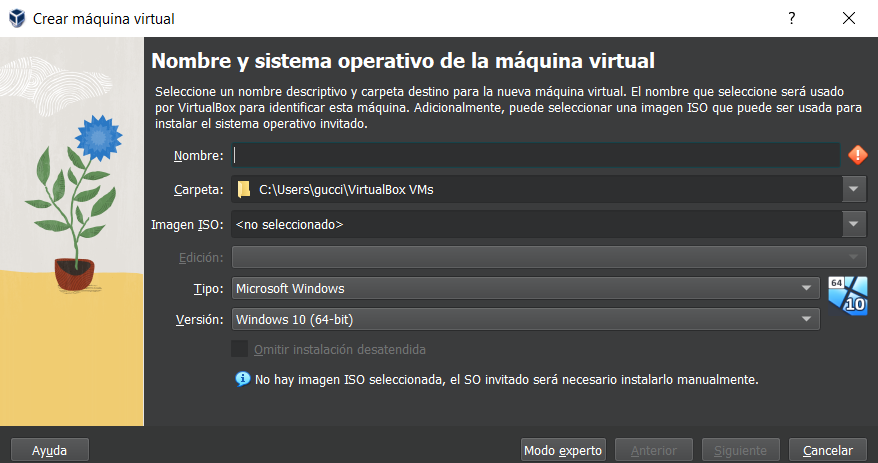
\includegraphics[width=0.4\linewidth]{MVU.png}
        \captionof{figure}{Creación Máquina Virtual}
        \label{fig:etiqueta}
    \end{minipage}\\

    \item[\textbf{3.3}] Revisamos las especificaciones de nuestro computador, para seguir con la creación de nuestra máquina virtual.

    \begin{minipage}{\linewidth}
        \centering
        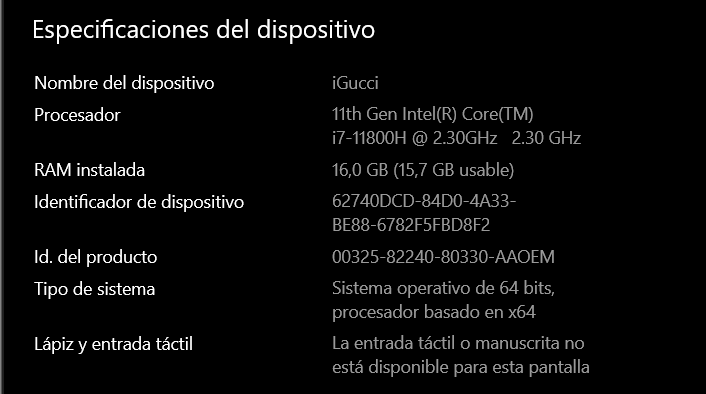
\includegraphics[width=0.4\linewidth]{Especificaciones.png}
        \captionof{figure}{Especificaciones del Computador}
        \label{fig:etiqueta}
    \end{minipage}\\

    \item[\textbf{3.4}] Al revisar nuestras especificaciones seguimos con la creación de la máquina, en la cual tenemos que señalar la memoria base y los procesadores.

    \begin{minipage}{\linewidth}
        \centering
        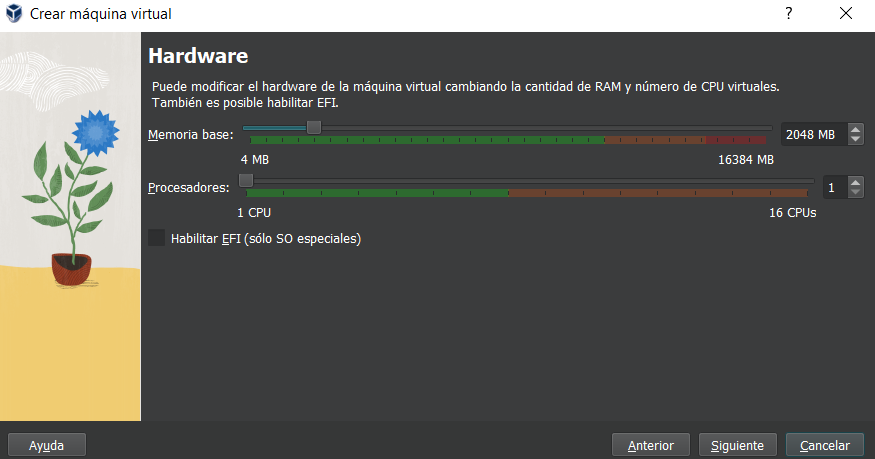
\includegraphics[width=0.4\linewidth]{H.Wmv.png}
        \captionof{figure}{Hardware}
        \label{fig:etiqueta}
    \end{minipage}\\

     \item[\textbf{3.5}] Después de terminada la instalación y configuración ya podremos usar la máquina virtual de Ubuntu.

    \begin{minipage}{\linewidth}
        \centering
        
\includegraphics[width=0.4\linewidth]{Ubt.png}
        \captionof{figure}{Ubt}
        \label{fig:etiqueta}
    \end{minipage}\\
    


    % Añade más pasos si es necesario
\end{enumerate}

\subsection*{Conclusiones}
\begin{itemize}
  \item La creación de una máquina virtual en Ubuntu es un proceso eficiente y beneficioso para diversos fines. Al crear una máquina virtual, se logra un entorno virtualizado que permite ejecutar diferentes sistemas operativos y aplicaciones en una sola máquina física. Esto brinda flexibilidad, escalabilidad y seguridad.
  \item Tener en cuenta las especificaciones de cada computador para el correcto funcionamiento de la maquina virtual que se va a crear.
\end{itemize}

\subsection*{Referencias}
Download Ubuntu Desktop | Download | Ubuntu. (s.f.). Ubuntu. https://ubuntu.com/download/desktop 
\end{enumerate}

\section{Laboratorio 2}
\subsection{Comandos básicos de Linux}

\textbf{Objetivos:}
\begin{itemize}
  \item Al final la sesión el estudiante aprenderá a obtener ayuda en línea para obtendrá ayuda en línea para aprehender cualquier comando que necesite.
  \item Al finalizar esta clase el estudiante será capas de navegar por todo el filesystem , prender y apagar la maquina.
\end{itemize}

\textbf{Recursos:}
\begin{itemize}
  \item PC
  \item Windows 10
  \item VirtualBox
  \item Ubuntu - .ISO
\end{itemize}

\subsection*{Desarrollo}
En esta practica de laboratorio aprenderemos los comandos basicos de Linux con la finalidad de adentrarnos y familiarizarnos. 
\begin{enumerate}
  \item[\textbf{1.}] \textbf{Comandos para tareas básicas de Linux} 
  \begin{itemize}
      \item hostname: Manual en linea.
      \item pwd: Muestra el directorio actual.
      \item clear: limpiar pantalla
      \item ls: Lista el contenido de una carpeta.
      \item cd: Cambia de directorio.
      \item cat: Muestra el contenido de un archivo.
      \item mkdir: Crea un nuevo directorio.
      \item rm: Elimina archivos o directorios.
      \item history: Muestra el historial de comandos ejecutados.
      \item tar: Archiva o descomprime archivos.
      \item sudo: Ejecuta un comando con privilegios de superusuario.
      \item top: Muestra los procesos que están consumiendo más recursos del sistema.
      \item df: Muestra el espacio libre y utilizado en los sistemas de archivos.
      \item ping: Verifica la conectividad de red con un host remoto.
      \item ls -a: Lista archivos y directorios, incluyendo los ocultos.
      \item info: Proporciona información adicional sobre el sistema y comandos.
      \item help: Muestra información de ayuda sobre el comando.
       \item date: Muestra la fecha y la hora actuales.
       \item who: Muestra información sobre los usuarios conectados.
     \item whoami: Muestra el nombre de usuario actual.
  \end{itemize}
        \begin{minipage}{\linewidth}
        \centering
        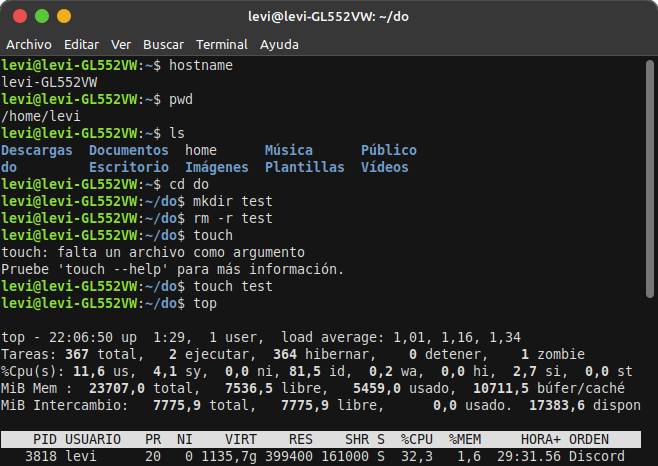
\includegraphics[width=0.6\linewidth]{basico.png}
        \captionof{figure}{Comando basicos de linux}
        \label{fig:etiqueta}
    \end{minipage}\\
            \begin{minipage}{\linewidth}
        \centering
        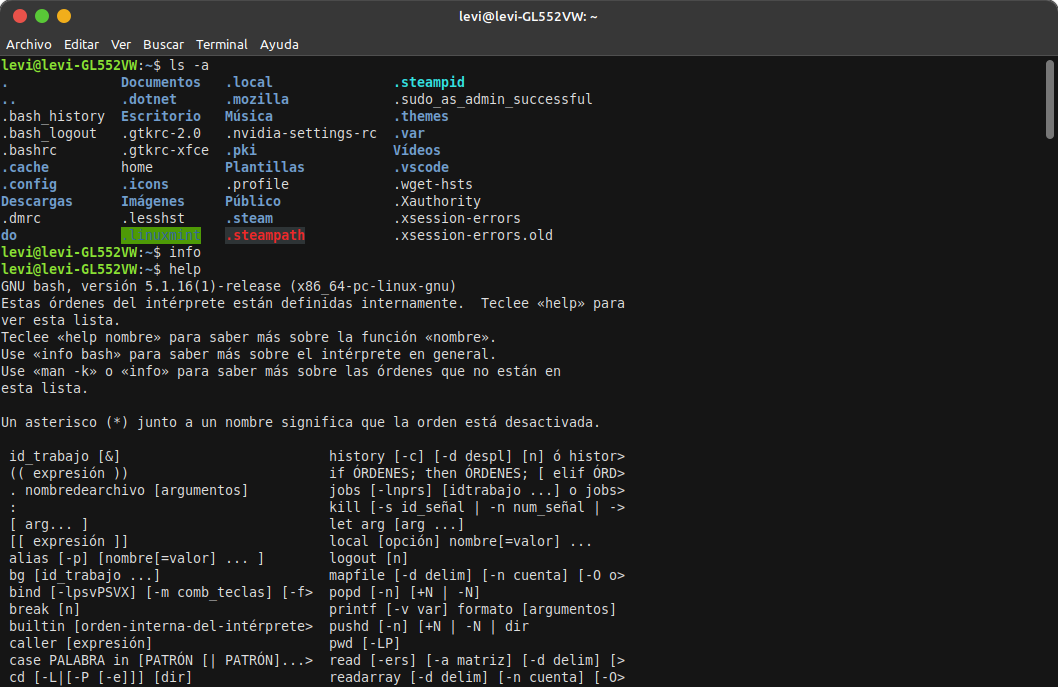
\includegraphics[width=0.6\linewidth]{ls.png}
        \captionof{figure}{Comando basicos de linux}
        \label{fig:etiqueta}
    \end{minipage}\\
            \begin{minipage}{\linewidth}
        \centering
        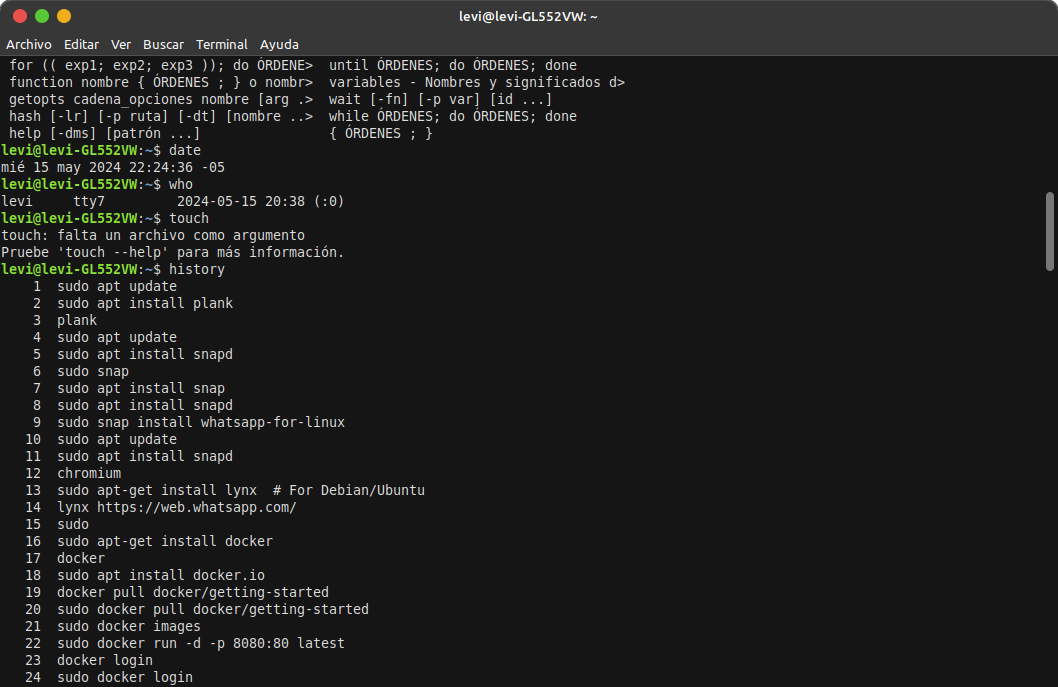
\includegraphics[width=0.6\linewidth]{ls1.png}
        \captionof{figure}{Comando basicos de linux}
        \label{fig:etiqueta}
    \end{minipage}\\
  \item[\textbf{2.}] \textbf{Comandos para ver las versiones: }
  \begin{itemize}
  \item \textbf{uname -v:}  Este comando devuelve la versión del kernel (núcleo) del sistema operativo. Proporciona detalles sobre la versión del kernel que está actualmente en ejecución.
  \item \textbf{uname -s:}  Devuelve el nombre del sistema operativo. 
  \item \textbf{ uname -r: } Proporciona la versión del kernel. Muestra la versión específica del kernel que está en ejecución.
  \item \textbf{uname -o: } Este comando devuelve el nombre del sistema operativo 
  \item \textbf{uname -p: } Proporciona el tipo de procesador o arquitectura de la máquina.  
\end{itemize}
    \begin{minipage}{\linewidth}
        \centering
        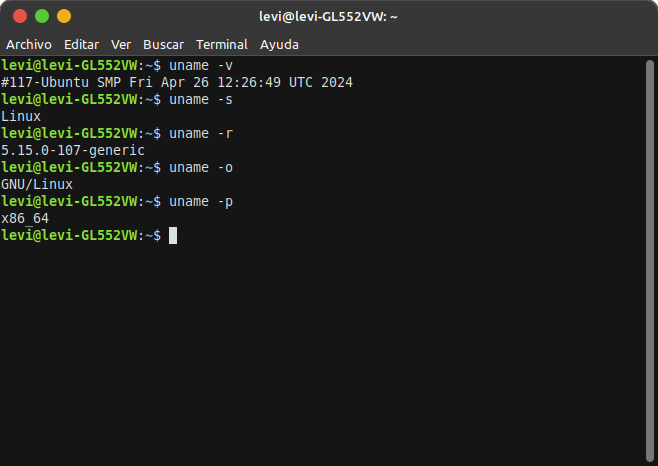
\includegraphics[width=0.6\linewidth]{uname.png}
        \captionof{figure}{Comandos en Linux}
        \label{fig:etiqueta}
    \end{minipage}\\
  
  \item[\textbf{3.}] \textbf{Comando para el manual de texto} 
  \begin{itemize}
      \item\textbf{man uname: }  Se utiliza para mostrar el manual de la utilidad uname. La utilidad uname proporciona información sobre el sistema operativo en el que se esta trabajando. Al ejecutar man uname, accedemos a la página del manual que describe en detalle cómo usar este comando y qué opciones puedes utilizar con él. 
  \end{itemize}
      \begin{minipage}{\linewidth}
        \centering
        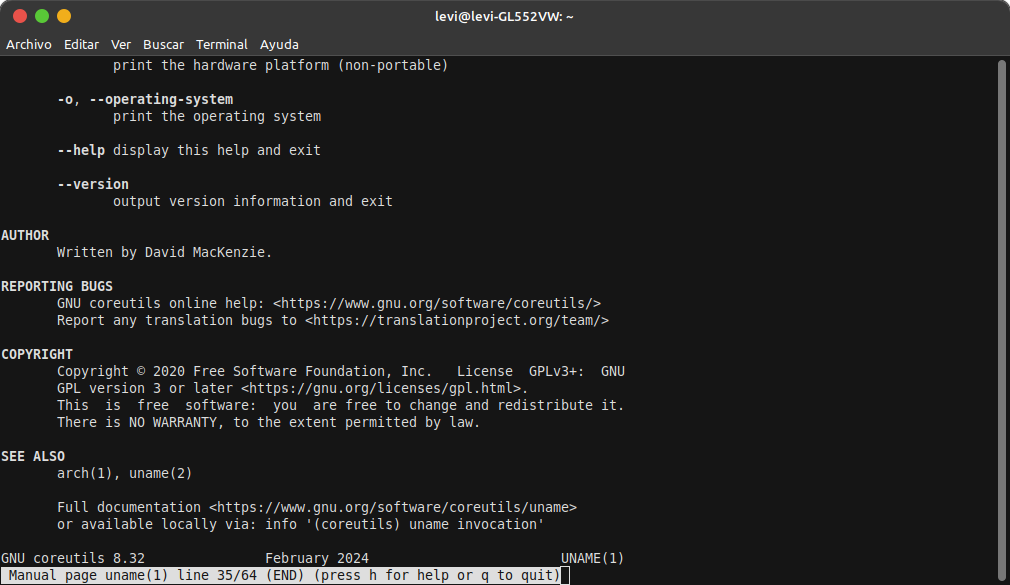
\includegraphics[width=0.6\linewidth]{manuname.png}
        \captionof{figure}{Comando man uname}
        \label{fig:etiqueta}
    \end{minipage}\\

  \item[\textbf{4.}] \textbf{Comandos para navegación de directorios} 


    Como se logra observar en la figura 1.13,se están ejecutando una serie de comandos para navegar por el sistema de archivos. A continuación se detalla lo que se está haciendo en cada paso:
  \begin{itemize}
      \item 'pwd': Muestra el directorio actual, que es '/home/levi'.
      \item 'cd ..': Cambia al directorio padre, por lo que el directorio actual se convierte en '/home'.
      \item pwd: Muestra el directorio actual, que es "/home".
      \item 'cd ..': Cambia al directorio padre, por lo que el directorio actual se convierte en "/" (raíz del sistema de archivos).
      \item 'pwd': Muestra el directorio actual, que es '/' (raíz del sistema de archivos).
      \item 'cd /home/lrvi/': Cambia al directorio '/home/levi/'.
      \item El prompt cambia a \texttt{levi@levi-GL552VW: \textdollar}, lo que indica que el directorio actual es \texttt{"/home/levi"}.
  \end{itemize}
        \begin{minipage}{\linewidth}
        \centering
        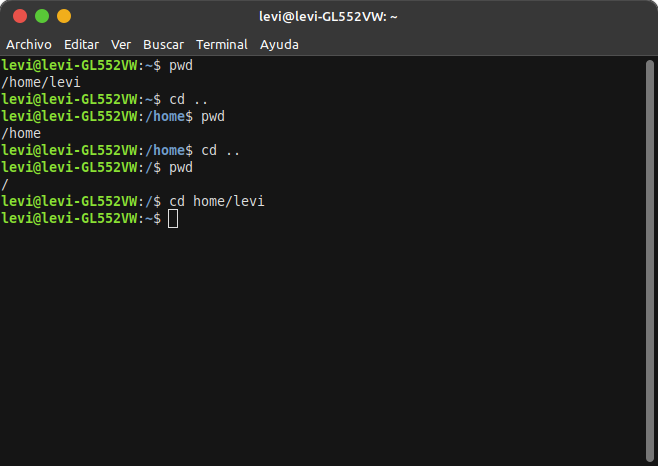
\includegraphics[width=0.6\linewidth]{directorios.png}
        \captionof{figure}{Navegación de directorios}
        \label{fig:etiqueta}
    \end{minipage}\\
  Adicionalmente, se puede ver la estructura de directorios de manera gráfica con el comando 'tree'. A continuación se realiza una breve descripción de los comandos de tree:
  \begin{itemize}
      \item\textbf{sudo apt-get install tree: } Comando que instala el comando tree, ya que este comando no viene instalado por defecto en ubuntu.
      \item\textbf{tree: } Imprime la estructura de los directorios y archivos en forma de arbol lo que facilita la visualización de la jerarquía de los directorios del sistema operativo. Además, el comando tree permite listar los directorios de los dispositivos externos. Al ejecutar el comando tree sin opciones, se mostrará la estructura de directorios a partir del directorio actual.
      \item\textbf{tree -L 1: } Muestra la estructura de directorios del directorio actual hasta un nivel de profundidad específico, en este caso, un nivel. La opción '-L' seguida de un número indica el nivel de profundidad que se desea mostrar en el árbol de directorios. Al utilizar '-L 1', se mostrará únicamente el contenido del directorio actual, sin incluir subdirectorios. Esto es útil para obtener una vista rápida de la estructura de directorios en el directorio actual sin adentrarse en subdirectorios.
      \item \textbf{tree -L 1 \textbar{} more:} Muestra la estructura de directorios del directorio actual hasta un nivel de profundidad específico. Al utilizar '\texttt{\textbar{}}' (pipe) y el comando \texttt{more}, la salida se visualiza de manera controlada, permitiendo desplazarse por el contenido página por página. Esto es útil para obtener una vista rápida y organizada de la estructura de directorios en el directorio actual sin adentrarse en subdirectorios.

      \begin{minipage}{\linewidth}
        \centering
        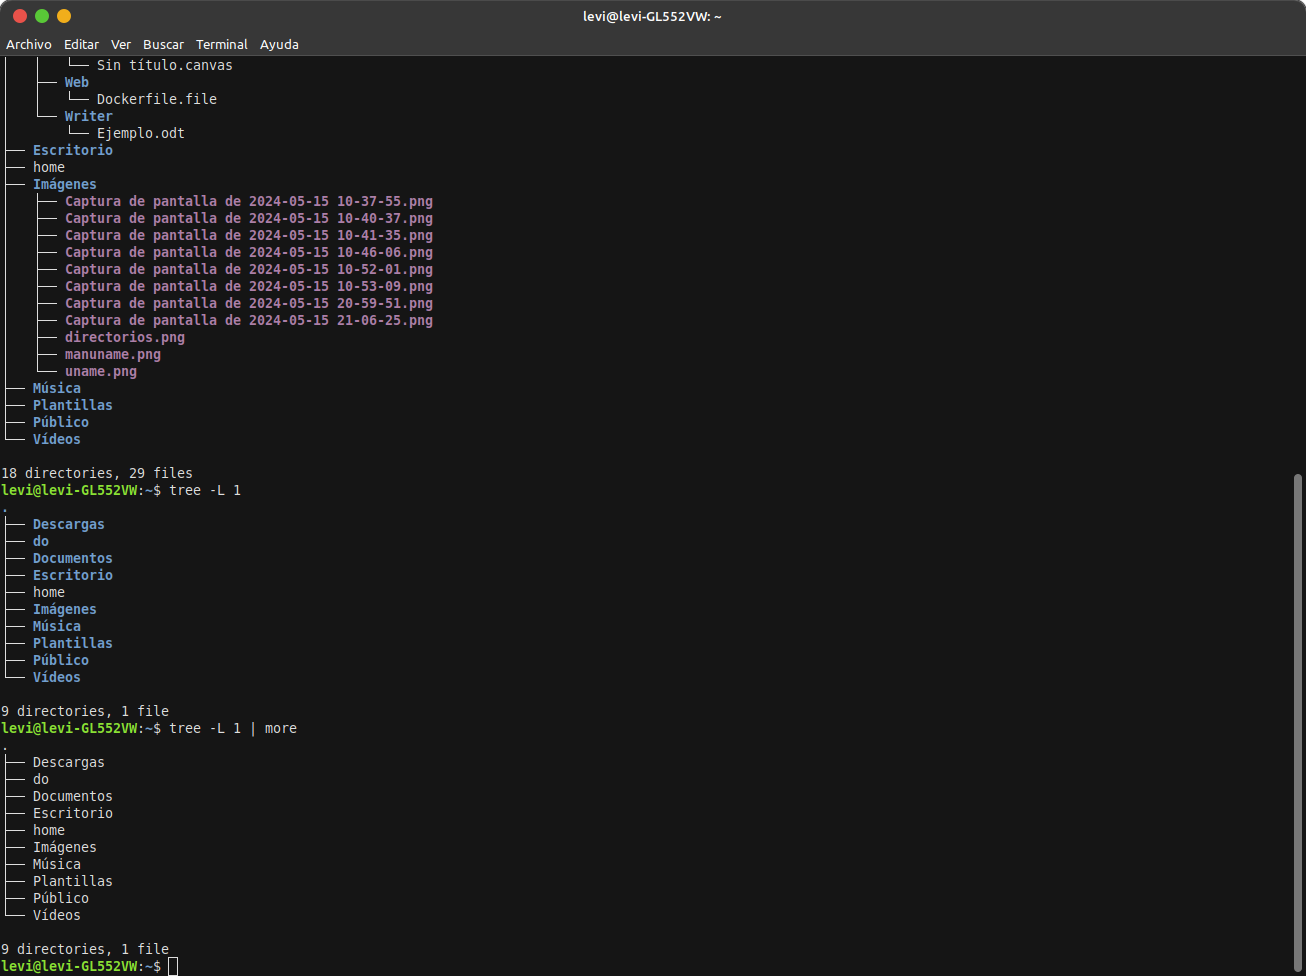
\includegraphics[width=1\linewidth]{tree.png}
        \captionof{figure}{Vista del comando 'tree -L 1'}
        \label{fig:etiqueta}
    \end{minipage}\\
    
    \item \textbf{history}: Muestra el historial de comandos previamente ejecutados en una sesión.
      
      
      
  \end{itemize}
  \item[\textbf{6.}] \textbf{Comando para apagar la maquina virtual} 
  \begin{itemize}
      \item shutdown -h now
  \end{itemize}
      \begin{minipage}{\linewidth}
        \centering
        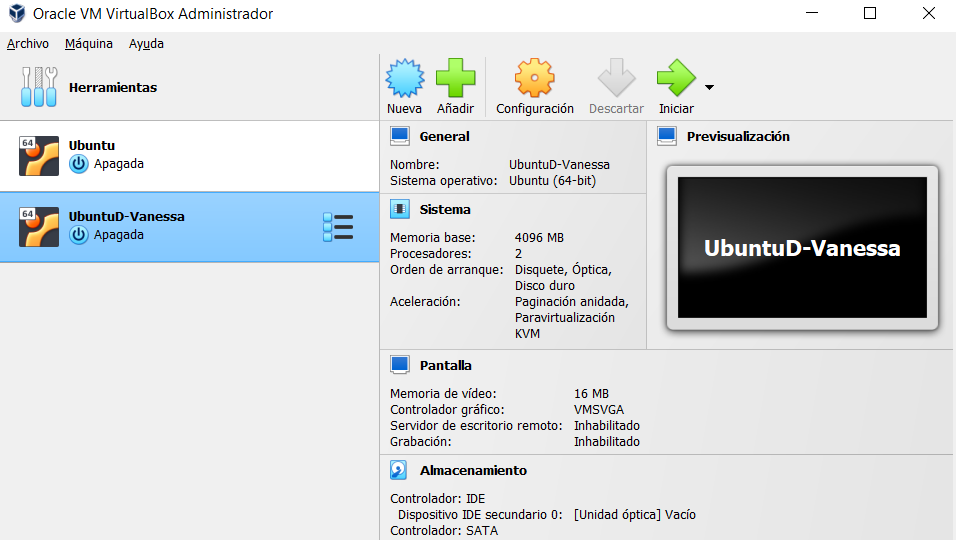
\includegraphics[width=0.5\linewidth]{comandoapagar.png}
        \captionof{figure}{Comando para apagar la maquina virtual}
        \label{fig:etiqueta}
    \end{minipage}\\

  

\subsection*{Conclusiones}
\begin{itemize}
  \item Los comandos básicos de Linux son fundamentales para la administración y manipulación de archivos y directorios en un sistema operativo, estos comandos permiten a los usuarios realizar tareas como crear, copiar, mover y eliminar archivos, así como navegar por la estructura de directorios del sistema.
  \item Los comandos "uname -v", "-s", "-r", "-o" y "-p" son herramientas útiles para obtener información específica sobre el sistema operativo y el kernel en un sistema Linux.
  \item El comando "man uname" es una herramienta útil para obtener información detallada sobre el comando "uname" y aprovechar al máximo sus funcionalidades en un sistema Linux.
\end{itemize}

\subsection*{Referencias}
Equipo editorial de IONOS. (2023, 22 agosto). Comandos de Linux. IONOS Digital Guide. 

\end{enumerate}
\newpage

\section{ Laboratorio 3}
\subsection{Gestión de archivos y directorios en Linux}

\textbf{Objetivos:}
\begin{itemize}
  \item Identificar el sistema de archivos Linux
  \item Manipular archivos y directorios 

\end{itemize}

\textbf{Recursos:}
\begin{itemize}
  \item PC
  \item MS-Windows
  \item VirtualBox
  \item Ubuntu - .ISO
\end{itemize}

\subsection*{Desarrollo}
La gestión de archivos en Linux es un aspecto fundamental del sistema operativo, ya que proporciona herramientas y comandos para crear, remover, renombrar, editar, visualizar y eliminar archivos y directorios. Con su estructura jerárquica de directorios, Linux permite a los usuarios y administradores organizar la información de manera eficiente. 

\subsection*{Gestion de archivos} 
\begin{enumerate}
    \item [\textbf{1.}] \textbf{Comando mkdir}: Con este comando podemos crear el directorio donde se van a alamcenar los arhivos de la practica.
    \begin{figure}[htb]
    \centering
    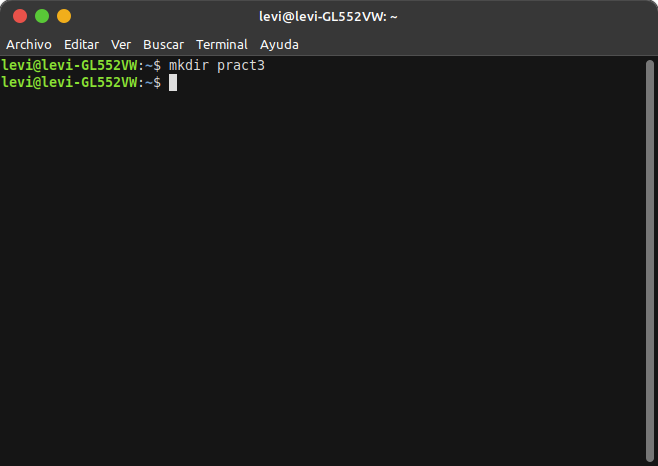
\includegraphics[width=0.5\linewidth]{introduccion/Lab3/mkdir.png}
    \caption{Comando mkdir}
   \label{fig:etiqueta}
    \end{figure}
    \item [\textbf{2.}] \textbf{Comando cd}: Con este comando podemos acceder al directorio que hemos creado.
    \begin{figure}[htb]
    \centering
    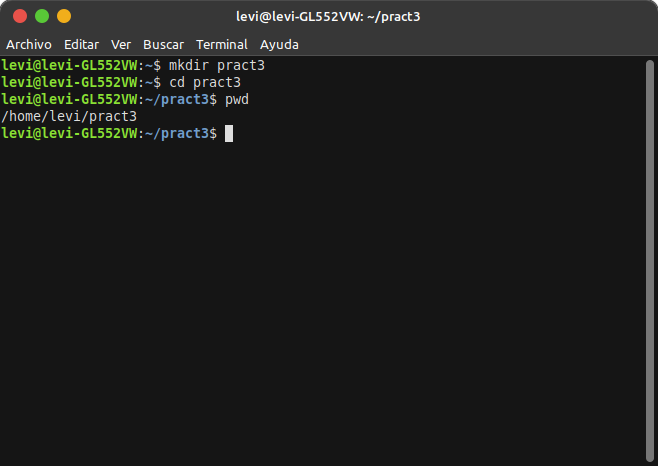
\includegraphics[width=0.6\linewidth]{introduccion/Lab3/cdpwd.png}
    \caption{Comando cd y pwd}
   \label{fig:etiqueta}
    \end{figure}
    \newpage
    \item [\textbf{3.}] \textbf{Comando touch}: Con este comando podemos crear un archivo el cual va a estar vacio. 
    \begin{figure}[htb]
    \centering
    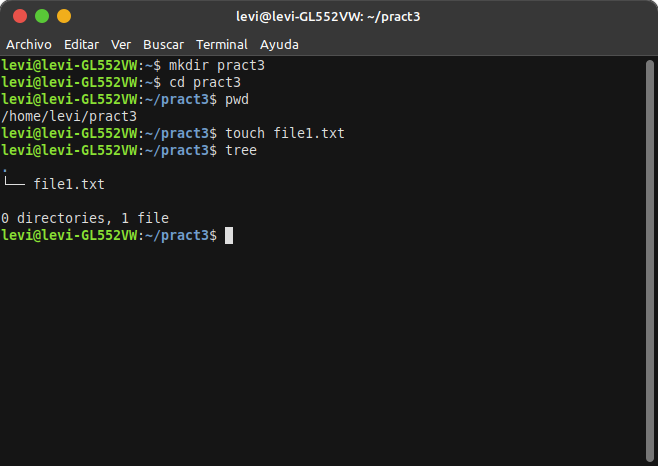
\includegraphics[width=0.6\linewidth]{introduccion/Lab3/touch.png}
    \caption{Comando touch}
   \label{fig:etiqueta}
    \end{figure}
    \newpage
    \item [\textbf{4.}] \textbf{Comando ls-l}: Este comando se utiliza para mostrar el contenido de un directorio.
  
  \begin{figure}[htb]
    \centering
    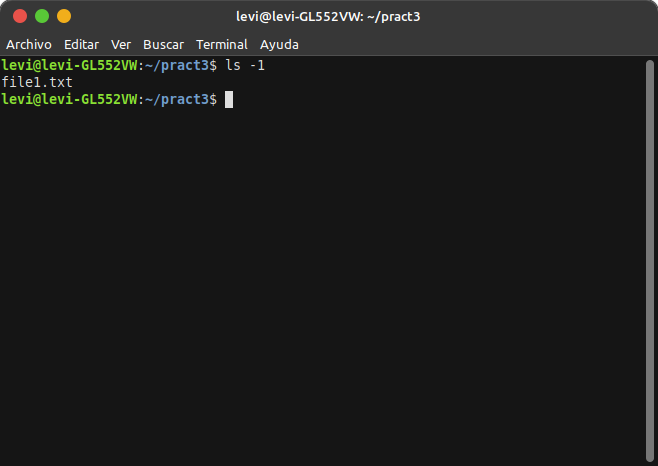
\includegraphics[width=0.6\linewidth]{introduccion/Lab3/cls.png}
    \caption{Comando ls -l}
   \label{fig:etiqueta}

    \end{figure}
        \item [\textbf{5.}] \textbf{Comando cat}: Este comando nos permite realizar el redirecionamiento de informacion al archivo que creamos
    \begin{figure}[htb]
    \centering
    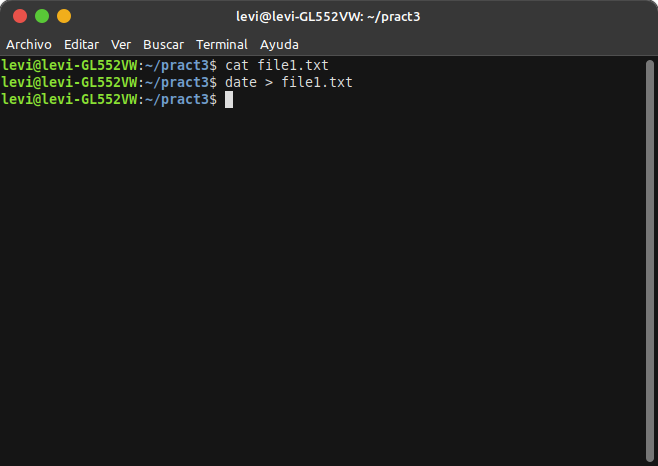
\includegraphics[width=0.6\linewidth]{introduccion/Lab3/catdate.png}
    \caption{Comando cat y redirecionamiento de data al file1.txt}
   \label{fig:etiqueta}
    \end{figure}
    \newpage
    \item [\textbf{6.}] \textbf{Comando cal}: Permite observar la fecha que deseamos, pero para utilizar primero tenemos que instalarnos con el siguiente comando: sudo apt-get -y install ncal 
    \begin{figure}[htb]
    \centering
    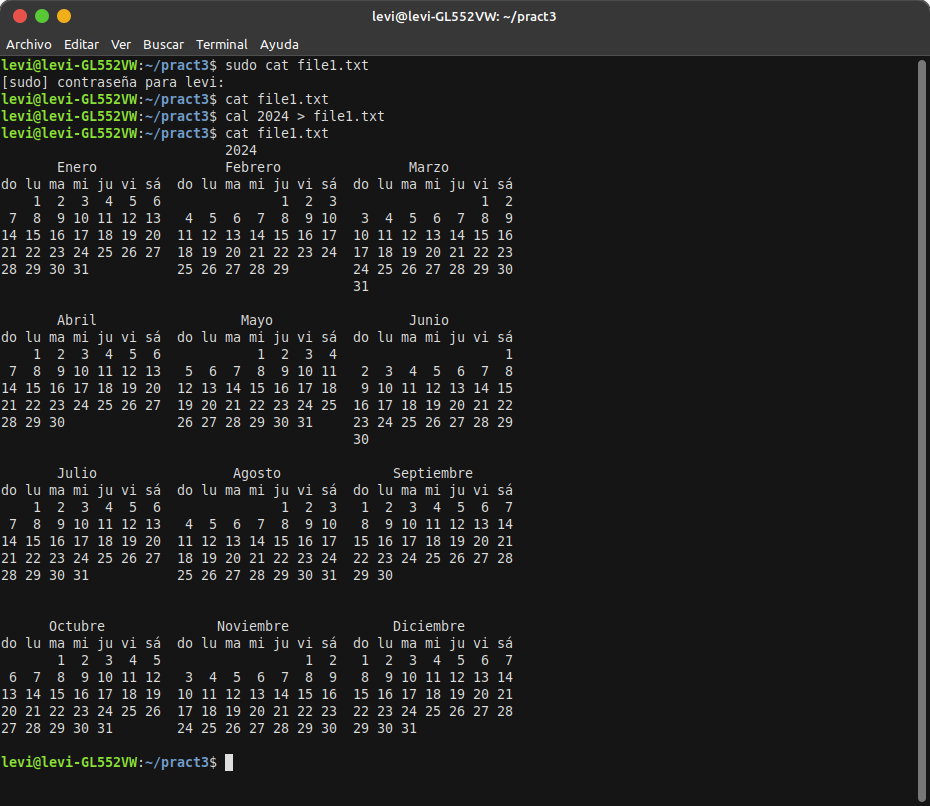
\includegraphics[width=0.5\linewidth]{introduccion/Lab3/cal.png}
    \caption{Comando cal}
   \label{fig:etiqueta}
    \end{figure}

    \item [\textbf{7.}] \textbf{Comando diff}: Este comando permite comparar el contenido de los archivos.  
    \begin{figure}[htb]
    \centering
    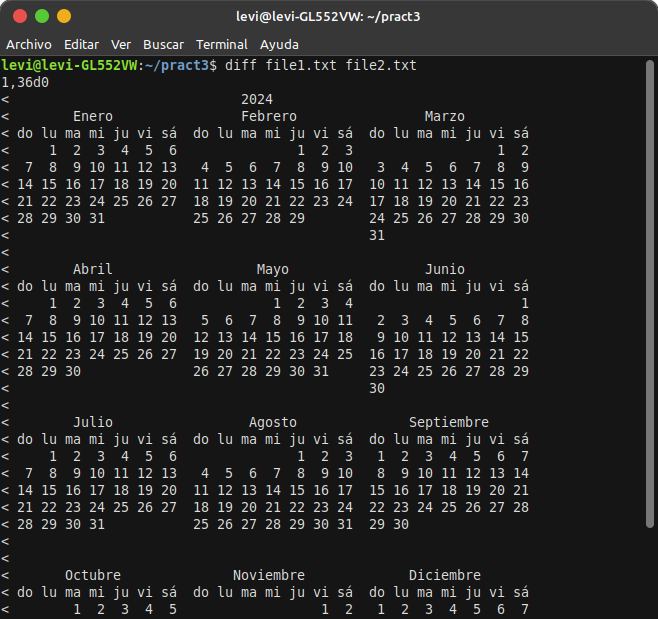
\includegraphics[width=0.5\textwidth]{introduccion/Lab3/diff.png}
    \caption{Comando diff}
   \label{fig:etiqueta}
    \end{figure}
    \newpage
      \item [\textbf{8.}] \textbf{Comando cp}: Este comando permite copiar el contenido de los archivos.  

\end{enumerate}

\subsection*{Conclusiones}
\begin{itemize}
  \item En este laboratorio se observa la importancia de la gestion de archivos y directorios en Linux ya que es fundamental para organizar y administrar información.
  \item LLos comandos mencionados anteriormente son herramientas impoetantes que permiten manipular y controlar los archivos y directorios de manera eficiente.
\end{itemize}

\subsection*{Referencias}

Marco. (s.f.). \textit{MANEJO DE ARCHIVOS y DIRECTORIOS a TRAVÉS DE COMANDOS.} \url{https://www.investigacion.frc.utn.edu.ar/labsis/publicaciones/apunte_linux/mmad.html}

10 – Comandos básicos para gestión de archivos. (s.f.). \url{https://www.valenciatech.com/10-comandos-basicos-para-gestion-de-archivos/}
\break
\newpage

\section{ Laboratorio 4}
\subsection{Programación en Shell Script}

\textbf{Objetivos:}
\begin{itemize}
  \item   El estudiante comprendera en que consiste este lenguaje de de programación.
  \item El estudiante automatizara procesos programados con shell script.  
  \item El estudiante podrá crear comandos Linux propios.
\end{itemize}

\textbf{Recursos:}
\begin{itemize}
  \item PC
  \item MS-Windows
  \item VirtualBox
  \item Ubuntu - .ISO
\end{itemize}

\subsection*{Desarrollo}
Shell Script es un lenguaje de programación interprete de comandos que tiene como objetivo automatizar procesos mediante la creación secuencias de código contenidos dentro de un programa llamado script. Los scripts de shell pueden ser utilizados para realizar una amplia gama de tareas, como el procesamiento de archivos, la administración del sistema, la manipulación de datos y la automatización de flujos de trabajo.

\vspace{10pt}

\textbf{Tipos de shell script}
\begin{itemize}
  \item\textbf{C Shell: }El shell C es un intérprete de mandatos interactivo y un lenguaje de programación de mandatos. Utiliza una sintaxis que es similar al lenguaje de programación C.
  \item\textbf{Korn Shell: }El shell Korn (mandato ksh) es compatible con las versiones anteriores del shell Bourne (mandato bsh) y contiene la mayoría de las características del shell Bourne así como algunas de las mejores características del shell C.
  \item\textbf{BASH Shell (Bourne Again Shell): } Es una mejora del Bourne Shell y es el shell predeterminado en la mayoría de las distribuciones de Linux.
\end{itemize}

\textbf{Tipos de editores}
\begin{itemize}
  \item\textbf{Vin: }Vim es la version mejorada del editor de texto Vi. La principal característica tanto de Vim como de Vi consiste en que disponen de diferentes modos entre los que se alterna para realizar ciertas operaciones.
La aternacia de estos modos ofrecen una gran versatilidad a la hora de editar el codigo que nos mejora enormente la eficiencia de la edicion del texto .
  \item\textbf{Nano: }GNU nano es un editor de textos de comandos muy extendido que se incluye en la mayoría de las distribuciones de Linux. La interfaz es comparable a la de los editores de texto con interfaz gráfica, lo que hace que nano sea una opción muy apreciada por quienes consideran que los comandos de vi o emacs no son intuitivos.

\end{itemize}
\vspace{10pt}

  \textbf{Requerimientos}
  \begin{itemize}
  \item Editor de texto plano nano.
  \item Crear el programa con extensión sh.
  \item Ejecutar el programa.
\end{itemize}

\vspace{10pt}

Ejercicio 1
Primer progama 

\begin{lstlisting}
#!/bin/bash
#Program: Hello World
#Author: Gustavo Aguas y Sebastián Paucar
#Date: Mayo 22th, 2024
echo "Hello World"
echo "I love Linux"
echo "Version: "
# End Program
\end{lstlisting}
 \begin{figure}[htb]
    \centering
     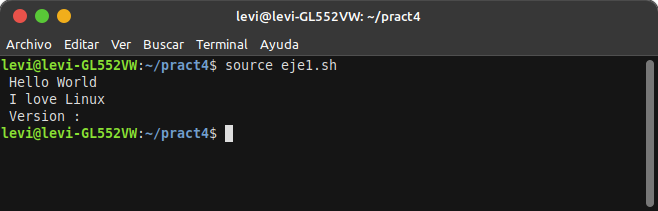
\includegraphics[width=0.8\linewidth]{introduccion/Lab4/eje1.png}
    \caption{Programa Shell: Hello World}
   \label{fig:etiqueta}
    \end{figure}
\vspace{10pt}

Ejercicio 2
Permitir visualizar el arbol de directorios de Linux y el estado de archivos de mi carpeta

The Kernel version
\begin{lstlisting}
#!/bin/bash
#Program: The kernel version
#Author: Gustavo Aguas y Sebastian Paucar
#Date: Nov 22th, 2023
clear
echo "The kernel information"
echo "The kernel version"; uname -v
echo "The kernel realease": uname -r
echo "The kernel distro"; uname -o
echo "The kernel procesor" ; uname -p
echo "Bye,I love Linux"
\end{lstlisting}
\begin{figure}[htb]
    \centering
     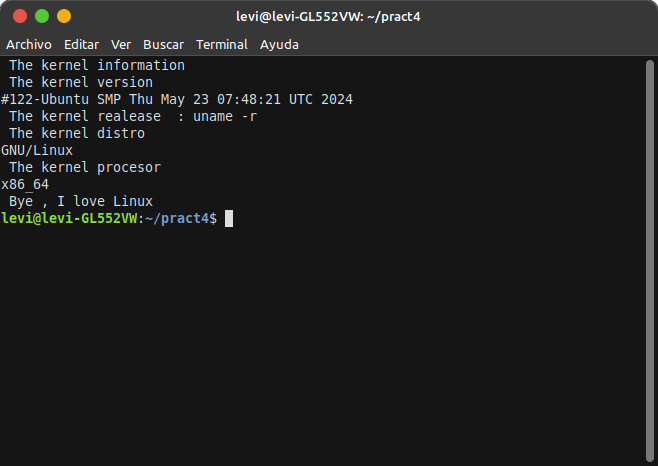
\includegraphics[width=0.8\linewidth]{introduccion/Lab4/ejerKernel.png}
    \caption{Programa Shell: The kernel version}
   \label{fig:etiqueta}
    \end{figure}
    
\vspace{10pt}
\newpage
\subsection*{Conclusiones}
\begin{itemize}
  \item Los scripts de shell permiten a los usuarios crear secuencias de comandos para llevar a cabo tareas específicas de manera eficiente.
  \item Es importante comprender los conceptos básicos de la programación en shell, como las estructuras de control, las variables y los comandos integrados,para poder aprovechar al máximo esta herramienta.
\end{itemize}
\newpage
\section{Laboratorio 5}
\subsection{Tema: Permisos de archivos y directorios}

\textbf{Objetivos:}
\begin{itemize}
  \item Comprender que los archivos y directorios requieren de permisos de escritura(r), lectura(w) y ejecución(x) para su utilización.
  \item Aprender a asignar/quitar permisos 
  \end{itemize}
\subsection*{Desarrollo}
La estructura de un archivo se compone de la siguiente manera:
\begin{figure}[htb]
  \centering
  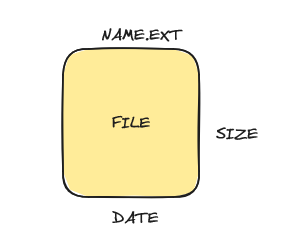
\includegraphics[width=0.5\linewidth]{introduccion/lab6/archivo_estruc.PNG}
  \caption{Estructura de un archivo}
  \label{fig:etiqueta}
\end{figure}


Los tipos de archivos a los que se les puede asignar permisos son los archivos, directorios y link, se los puede identificar por -,d y l respectivamente:

\begin{itemize}
  \item -	rwx -wx r—permisos1.sh -> file
  \item d r-x rwx rwx America -> directorios
  \item l r-x rwx rwx America -> link
\end{itemize}
\subsection*{Tipos de permisos:}
\begin{itemize}
  \item r: read
  \item w: write
  \item x: execution 
\end{itemize}
\subsection*{Tipos de archivos:}
\begin{itemize}
  \item -: file
  \item d: directory
  \item l: link
  \item p: pipe
  \item s: socket
  \item b: block
\end{itemize}
\subsection*{Tipos de propietarios:}
\begin{itemize}
  \item u: user
  \item g: group
  \item o: others 
  \item a: all
\end{itemize}

\subsection*{Comandos Linux para otorgar permisos:}
\begin{itemize}
  \item chmod: Permite otorgar permichos a los archivos y directorios pero solo del u propietario.
  \item chgrp: 
  \item chown
\end{itemize}

\subsection*{Formas de otorgar permisos:}

    \item Numérica (Absoluta)
        \begin{center}
        \begin{tabular}{|c|c|c|c|}
        \hline
        \textbf{Número} & \textbf{r (read)} & \textbf{w (write)} & \textbf{x (execute)} \\
        \hline
        0 & 0 & 0 & 0 \\
        1 & 0 & 0 & 1 \\
        2 & 0 & 1 & 0 \\
        3 & 0 & 1 & 1 \\
        4 & 1 & 0 & 0 \\
        5 & 1 & 0 & 1 \\
        6 & 1 & 1 & 0 \\
        7 & 1 & 1 & 1 \\
        \hline
        \end{tabular}
        \captionof{table}{Tabla de permisos en notación octal para archivos en Linux.}
        \end{center}
        
        \subsection*{Ejercicio1:  Otorgue permisos de r al u/g, permiso de w al u/o, permiso de ejecucion a todos}
        \begin{itemize}
        \item chmod 753 file100
        \item 111 101 011
        \end{itemize}

\begin{figure}
    \centering
    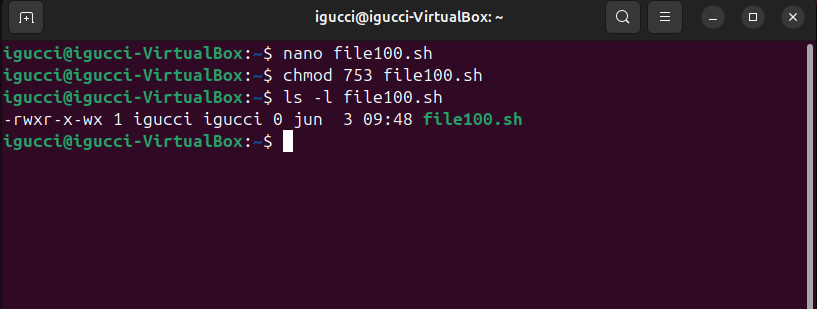
\includegraphics[width=1\linewidth]{file100.png}
    \caption{Ej 1}
\end{figure}
        \subsection*{Ejercicio2: Otorgue permisos  de lectura y escritura al archivo file101 solamente a usuarios propietarios y al grupo. Compruebe si puede modificar el archivo}
        \begin{itemize}
          \item chmod 660 file101
          \item 110 110 000
        \end{itemize}
        
        \subsection*{Ejercicio3: Dado el archivo file102 se despliegan los permisos 764. Cuales son los permisos asignados?}
        \begin{itemize}
          \item 111 110 100
          \item rwx rw- r--
        \end{itemize}
        
        \subsection*{Ejercicio4: Dado el archivo file103 otorgue permisos de lectura y ejecucion a todos}
        \begin{itemize}
          \item chmod 555 file103
          \item 101 101 101

        \end{itemize}
        
    \subsection*{Permisos Simbólicos}
        \begin{center}
        \begin{tabular}{|c|c|}
        \hline
        \textbf{Símbolo} & \textbf{Descripción} \\
        \hline
        u & user \\
        g & group \\
        o & others \\
        a & all \\
        r & read \\
        w & write \\
        x & execution \\
        = & asignación \\
        + & incremento \\
        - & eliminación \\
        \hline
        \end{tabular}
        \captionof{table}{Significado de los símbolos para otorgar permisos en Linux Shell.}
        \end{center}
        \subsection*{Ejercicio5: chmod a+x file104}
        \begin{itemize}
          \item añade el permiso de ejecución (\verb|x|) para el propietario, el grupo y otros,         manteniendo los permisos existentes de lectura (\verb|r|) y escritura (\verb|w|). 
\end{itemize}

        \subsection*{Ejercicio6: chmod go-x file105}
        \begin{itemize}
          \item elimina el permiso de ejecución (\verb|x|) para el grupo (\verb|g|) y otros (\verb|o|), mientras mantiene intactos los permisos de lectura (\verb|r|) y escritura (\verb|w|) que ya existían. No afecta a los permisos del propietario del archivo. 
        \end{itemize}
        
        \subsection*{Ejercicio8: chmod u-x, go-r file106}
        \begin{itemize}
          \item \verb|u-x|: Elimina el permiso de ejecución (\verb|x|) para el propietario (\verb|u|). 
          \item \verb|go-r|: Elimina el permiso de lectura (\verb|r|) para el grupo (\verb|g|) y otros (\verb|o|). 
        \end{itemize}

         \subsection*{Ejercicio9: chmod u-w, go-rwx file107}
        \begin{itemize}
          \item \verb|u-w|: Elimina el permiso de escritura (\verb|w|) para el propietario (\verb|u|). 
          \item \verb|go-rwx|: Elimina todos los permisos (lectura \verb|r|, escritura \verb|w| y ejecución \verb|x|) para el grupo (\verb|g|) y otros (\verb|o|). 
        \end{itemize}

         \subsection*{Ejercicio10: chmod a+r, u+w file108}
        \begin{itemize}
          \item \verb|a+r|: Agrega el permiso de lectura (\verb|r|) para todos los usuarios. 
          \item \verb|u+w|: Agrega el permiso de escritura (\verb|w|) solo para el propietario. 
        \end{itemize}

         \subsection*{Ejercicio11: chmod u-rw, g+w, o+x file109}
        \begin{itemize}
          \item \verb|u-rw|: Elimina los permisos de lectura y escritura para el propietario.
          \item  \verb|g+w|: Agrega el permiso de escritura para el grupo. 
          \item \verb|o+x|: Agrega el permiso de ejecución para otros. 
        \end{itemize}
        
       

\subsection{Funciones en Linux Shell}
Las funciones se encargan de:
\begin{itemize}
    \item Depurar 
    \item Organizar
    \item Modular
\end{itemize}
\subsection*{Ejemplo 1 de funciones en bash}
Calculadora de funciones
\begin{lstlisting}[language=bash, caption={Calculadora con funciones}]
#!/bin/bash

#Author: Gustavo Aguas y Sebastian Paucar

#Date: 03/06/2024

#Program: Calculadora con funciones

suma(){
        suma=$(echo "scale=2;$num1+$num2"|bc)
        echo "La suma es: $suma"
}

resta(){
        resta=$(echo "scale=2;$num1-$num2"|bc)
        echo "La resta es: $resta"
}

multiplicar(){
        multiplicar=$(echo "scale=2;$num1*$num2"|bc)
        echo "La multiplicacion: $multiplicar"
}

division(){
        divi=$(echo "scale=2;$num1/$num2"|bc)
        echo "La division: $divi"
}

potencia(){
        potencia=$(echo "scale=2;$num1^$num2"|bc)
        echo "La potencia es: $potencia"
}

echo "Ingrese el primer numero"
read num1;

echo "Ingrese el segundo numero"
read num2;

suma
resta
multiplicar
division
potencia

#I LOVE LINUX
\end{lstlisting}

\begin{figure}
    \centering
    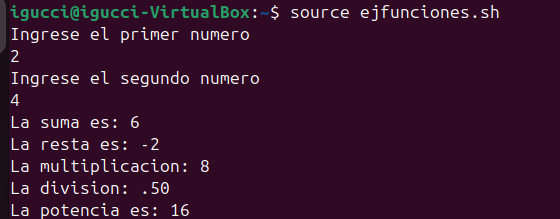
\includegraphics[width=1\linewidth]{ejfunc.png}
    \caption{Ej Funciones}
\end{figure}

\subsection*{Ejemplo 2 de funciones en bash}

\begin{lstlisting}[language=bash, caption={Calculadora con funciones}]
#!/bin/bash

#Author: Gustavo Aguas

#Date: 03/06/2024

#Program: Calculadora con funciones

suma(){
        suma=$(echo "scale=2;$num1+$num2"|bc)
        echo "La suma es: $suma"
}

resta(){
        resta=$(echo "scale=2;$num1-$num2"|bc)
        echo "La resta es: $resta"
}

multiplicar(){
        multiplicar=$(echo "scale=2;$num1*$num2"|bc)
        echo "La multiplicacion: $multiplicar"
}

division(){
        divi=$(echo "scale=2;$num1/$num2"|bc)
        echo "La division: $divi"
}

potencia(){
        potencia=$(echo "scale=2;$num1^$num2"|bc)
        echo "La potencia es: $potencia"
}

echo "Ingrese el primer numero"
read num1;

echo "Ingrese el segundo numero"
read num2;

suma
resta
multiplicar
division
potencia
\end{lstlisting}
\subsection*{Conclusiones}
\begin{itemize}  
  \item El conocer como otorgar permisos a ciertos directorios y archivos de Linux es de vital importancia para la seguridad de el sistema operativo donde se este trabajando, por lo que es una funcionalidad importante que incluye Ubuntu.
  \item La programación de funciones ayuda a quitar redundancias en instrucciones de en la programación de codigo, por lo que es útil para utilizar en mismo proceso en varias instrucciones del código.
\end{itemize}
\end{document}